% ============================================================
%  PRESENTACIÓN BEAMER – OpenMP: Ecuación de Poisson 2D
%  Camilo Huertas  ·  Sebastián Rodriguez
%  Universidad Distrital Francisco José de Caldas
% ============================================================
\documentclass[aspectratio=169,10pt,xcolor=table]{beamer}

% ─── TEMA BASE ───────────────────────────────────────────────
\usetheme{Madrid}
\usecolortheme{default}

% ─── PALETA DE COLORES PERSONALIZADA ────────────────────────
\definecolor{UDprimary}{RGB}{0,60,120}      % azul institucional
\definecolor{UDsecond}{RGB}{220,50,50}      % rojo acento
\definecolor{UDlight}{RGB}{230,240,255}     % fondo claro
\definecolor{UDdark}{RGB}{20,30,60}         % texto oscuro
\definecolor{codegreen}{rgb}{0,0.55,0.2}
\definecolor{codegray}{rgb}{0.5,0.5,0.5}
\definecolor{codepurple}{rgb}{0.50,0,0.70}
\definecolor{backcolour}{RGB}{245,245,240}

% ─── APLICAR COLORES AL TEMA ─────────────────────────────────
\setbeamercolor{palette primary}{bg=UDprimary,fg=white}
\setbeamercolor{palette secondary}{bg=UDdark,fg=white}
\setbeamercolor{palette tertiary}{bg=UDsecond,fg=white}
\setbeamercolor{palette quaternary}{bg=UDprimary!80,fg=white}
\setbeamercolor{structure}{fg=UDprimary}
\setbeamercolor{section in toc}{fg=UDprimary}
\setbeamercolor{block title}{bg=UDprimary,fg=white}
\setbeamercolor{block body}{bg=UDlight}
\setbeamercolor{block title alerted}{bg=UDsecond,fg=white}
\setbeamercolor{block body alerted}{bg=UDsecond!10}
\setbeamercolor{block title example}{bg=UDprimary!70,fg=white}
\setbeamercolor{block body example}{bg=UDprimary!8}
\setbeamercolor{frametitle}{bg=UDprimary,fg=white}
\setbeamercolor{title}{fg=white}
\setbeamercolor{author}{fg=UDlight}
\setbeamercolor{date}{fg=UDlight}
\setbeamercolor{itemize item}{fg=UDsecond}
\setbeamercolor{itemize subitem}{fg=UDprimary}
\setbeamercolor{enumerate item}{fg=UDsecond}

% ─── FUENTES ─────────────────────────────────────────────────
\usepackage[T1]{fontenc}
\usepackage[utf8]{inputenc}
\usepackage[spanish]{babel}
\usepackage{lmodern}
\usepackage{microtype}

% ─── PAQUETES ESENCIALES ─────────────────────────────────────
\usepackage{amsmath,amssymb}
\usepackage{graphicx}
\usepackage{booktabs}
\usepackage{tabularx}
\usepackage{multirow}
\usepackage{listings}
\usepackage{tikz}
\usetikzlibrary{shapes.geometric,arrows.meta,positioning,shadows,fit}

% ─── ESTILO DE CÓDIGO ────────────────────────────────────────
\lstdefinestyle{cppBeamer}{
  backgroundcolor=\color{backcolour},
  commentstyle=\color{codegreen}\itshape,
  keywordstyle=\color{UDprimary}\bfseries,
  keywordstyle=[2]\color{UDsecond}\bfseries,
  numberstyle=\tiny\color{codegray},
  stringstyle=\color{codepurple},
  basicstyle=\ttfamily\tiny, % <-- Reducido a \tiny para ahorrar espacio
  breakatwhitespace=false,
  breaklines=true,
  captionpos=b,
  keepspaces=true,
  numbers=left,
  numbersep=4pt,
  showspaces=false,
  showstringspaces=false,
  tabsize=2,
  frame=single,
  rulecolor=\color{UDprimary!40},
  xleftmargin=8pt,
  xrightmargin=4pt,
  literate={á}{{\'a}}1 {é}{{\'e}}1 {í}{{\'i}}1 {ó}{{\'o}}1 {ú}{{\'u}}1
           {Á}{{\'A}}1 {É}{{\'E}}1 {Í}{{\'I}}1 {Ó}{{\'O}}1 {Ú}{{\'U}}1
           {ñ}{{\~n}}1 {Ñ}{{\~N}}1
}
\lstset{style=cppBeamer}

% ─── PROGRESO Y NUMERACIÓN ───────────────────────────────────
\setbeamertemplate{navigation symbols}{}
\setbeamertemplate{footline}{%
  \leavevmode
  \hbox{%
    \begin{beamercolorbox}[wd=.30\paperwidth,ht=2.5ex,dp=1.125ex,leftskip=2pt]{palette secondary}%
      \usebeamerfont{author in head/foot}\insertshortauthor
    \end{beamercolorbox}%
    \begin{beamercolorbox}[wd=.45\paperwidth,ht=2.5ex,dp=1.125ex,center]{palette tertiary}%
      \usebeamerfont{title in head/foot}\insertshorttitle
    \end{beamercolorbox}%
    \begin{beamercolorbox}[wd=.25\paperwidth,ht=2.5ex,dp=1.125ex,rightskip=4pt plus1fil]{palette primary}%
      \usebeamerfont{date in head/foot}\hfill
      \insertframenumber{} / \inserttotalframenumber
    \end{beamercolorbox}%
  }%
}

\setbeamertemplate{headline}{%
  \begin{beamercolorbox}[ht=1.6ex,dp=0.4ex,wd=\paperwidth]{palette quaternary}%
    \hspace{6pt}{\tiny\color{white}\insertsectionhead}
    \hfill
    \begin{tikzpicture}[overlay]
      \fill[UDsecond] (0,0) rectangle (\paperwidth * \insertframenumber / \inserttotalframenumber, 0.8pt);
    \end{tikzpicture}
  \end{beamercolorbox}%
}

% ─── BULLETS PERSONALIZADOS ──────────────────────────────────
\setbeamertemplate{itemize item}{\color{UDsecond}\tiny\raisebox{1pt}{$\blacksquare$}}
\setbeamertemplate{itemize subitem}{\color{UDprimary}\tiny$\triangleright$}
\setbeamertemplate{enumerate item}{\color{UDsecond}\bfseries\insertenumlabel.}

% ─── METADATOS ───────────────────────────────────────────────
\title[OpenMP: Poisson 2D]{%
  \textbf{Paralelización con OpenMP}\\
  \large Ecuación de Poisson en 2D
}
\subtitle{Sistemas Distribuidos — Análisis de Escalabilidad HPC}
\author[Huertas · Rodriguez]{%
  \textbf{Camilo Huertas} \quad \textbf{Sebastián Rodriguez}\\
  {\small Programa Académico de Física}
}
\institute[UDFJC]{%
  Universidad Distrital Francisco José de Caldas\\
  {\small Docente: Carlos Andrés Gómez Vasco}
}
\date{24 de marzo de 2026}

% ============================================================
\begin{document}
% ============================================================

% ─── PORTADA ─────────────────────────────────────────────────
{
\setbeamertemplate{headline}{}
\setbeamertemplate{footline}{}
\begin{frame}[plain]
  \begin{tikzpicture}[remember picture,overlay]
    \fill[UDprimary] (current page.south west) rectangle (current page.north east);
    \fill[UDdark,opacity=0.5]
      (current page.south west) rectangle (current page.north east);
    \fill[UDsecond,opacity=0.85]
      ([xshift=-0.08\paperwidth]current page.north east) rectangle
      (current page.south east);
    \draw[UDlight,line width=1.5pt]
      ([yshift=-0.35\paperheight]current page.north west) --
      ([yshift=-0.35\paperheight,xshift=-0.08\paperwidth]current page.north east);
  \end{tikzpicture}

  \vspace{0.6cm}
  \begin{columns}[c]
    \column{0.18\textwidth}
       
\includegraphics[width=2.1cm]{../../imag/logoUD2.png}
    \column{0.82\textwidth}
      {\color{white}\Large\bfseries Paralelización con OpenMP}\\[4pt]
      {\color{UDsecond!80!white}\large\bfseries Ecuación de Poisson en 2D}\\[8pt]
      \color{white}\rule{0.9\textwidth}{0.4pt}\\[6pt]
      {\color{UDlight}\small Sistemas Distribuidos — Análisis de Escalabilidad HPC}\\[10pt]
      {\color{white}\normalsize\textbf{Camilo Huertas} \quad \textbf{Sebastián Rodriguez}}\\
      {\color{UDlight}\small Programa Académico de Física}\\[6pt]
      {\color{UDlight}\footnotesize Universidad Distrital Francisco José de Caldas}\\
      {\color{UDlight}\footnotesize Docente: Carlos Andrés Gómez Vasco \quad|\quad 24 de marzo de 2026}
  \end{columns}
\end{frame}
}

% ─── TABLA DE CONTENIDOS ─────────────────────────────────────
\begin{frame}{Contenido}
  \begin{columns}[t]
    \column{0.5\textwidth}
      \tableofcontents[sections={1-6}]
    \column{0.5\textwidth}
      \tableofcontents[sections={7-13}]
  \end{columns}
\end{frame}

% ============================================================
\section{Objetivo y Sistema HPC}
% ============================================================

% <-- Se añadió shrink=5 para autoajustar si el texto excede
\begin{frame}[shrink=5]{Objetivo del Proyecto}
  \begin{block}{Objetivo}
    Aplicar directivas de \textbf{OpenMP} para paralelizar la \textbf{Ecuación de Poisson 2D} (diferencias finitas). Se evaluará la \emph{escalabilidad}, cuellos de botella de memoria y límites de aceleración (Ley de Amdahl) mediante un barrido paramétrico masivo.
  \end{block}

  \vspace{0.1cm}
  \begin{columns}[t]
    \column{0.48\textwidth}
      \begin{block}{Problema Físico}
        La ecuación de Poisson en 2D:
        \vspace{-0.2cm}
        \[
          \frac{\partial^2 T}{\partial x^2}+\frac{\partial^2 T}{\partial y^2}=f(x,y)
        \]
        \vspace{-0.2cm}
        \begin{itemize}
          \item Término fuente $f(x,y)=4$.
          \item Esquema centrado \emph{in-place}.
          \item Tolerancia iterativa $\text{TOL}=10^{-6}$.
        \end{itemize}
      \end{block}
    \column{0.48\textwidth}
      \begin{block}{Directivas Evaluadas}
        \begin{itemize}
          \item \texttt{parallel for} + \texttt{reduction}
          \item \texttt{collapse(2)}
          \item \texttt{sections}
          \item \texttt{schedule(static)}
          \item \texttt{nowait}, \texttt{barrier}, \texttt{single}, \texttt{critical}
          \item \texttt{atomic} \quad | \quad \texttt{task}
        \end{itemize}
      \end{block}
  \end{columns}
\end{frame}

\begin{frame}{Especificaciones del Sistema HPC}
  \begin{columns}[c]
    \column{0.52\textwidth}
      \begin{block}{Hardware del Servidor}
        \renewcommand{\arraystretch}{0.9}
        \begin{tabular}{@{}ll@{}}
          \toprule
          \textbf{Componente} & \textbf{Especificación} \\
          \midrule
          Procesador & AMD Ryzen Threadripper 3990X \\
          Arquitectura & x86\_64 \\
          Núcleos / Hilos & \textbf{64} Físicos / \textbf{128} Lógicos \\
          Caché L3 & 256 MiB \\
          \bottomrule
        \end{tabular}
      \end{block}
      \vspace{0.2cm}
      \begin{block}{Relevancia Arquitectónica}
        La caché L3 de 256 MiB es clave: al superarse, el ancho de banda a la RAM se vuelve el \textbf{cuello de botella dominante} (Von Neumann).
      \end{block}
    \column{0.44\textwidth}
      \begin{block}{Metodología de Pruebas}
        \begin{itemize}
          \item Mallas: $50^2$, $100^2$, $200^2$ (hasta $512^2$)
          \item Hilos:\\ $p \in \{1,2,4,8,16,32,64,80\}$
        \end{itemize}
      \end{block}
      \begin{alertblock}{Sweet Spot Identificado}
        El máximo rendimiento se alcanza con \textbf{32 hilos}. Por encima de 64, el \emph{overhead} destruye el \emph{speedup}.
      \end{alertblock}
  \end{columns}
\end{frame}

% ============================================================
\section{Código Base Secuencial}
% ============================================================

\begin{frame}[fragile]{Código Base: Línea de Referencia}
  \begin{columns}[t]
    \column{0.56\textwidth}
      \begin{block}{Discretización (Diferencias Finitas)}
        \vspace{-0.3cm}
        \[
          T_{i,j}^{n+1}=
          \frac{(T_{i+1,j}+T_{i-1,j})k^2+(T_{i,j+1}+T_{i,j-1})h^2-f_{i,j}h^2k^2}
               {2(h^2+k^2)}
        \]
      \end{block}

\begin{lstlisting}[language=C++,caption={Bucle iterativo secuencial}]
while (delta > TOL) {
    delta = 0.0;
    for (int i = 1; i < M; ++i)
      for (int j = 1; j < N; ++j) {
        double T_old = T[i][j];
        T[i][j] = (((T[i+1][j]+T[i-1][j])*k*k)
          + ((T[i][j+1]+T[i][j-1])*h*h)
          - (source[i][j]*h*h*k*k))
          / (2.0*(h*h+k*k));
        double diff = abs(T[i][j]-T_old);
        if (diff > delta) delta = diff;
      }
    iterations++;
}
\end{lstlisting}
    \column{0.41\textwidth}
      \begin{block}{Resultados (1 hilo)}
        \scriptsize
        \renewcommand{\arraystretch}{0.9}
        \begin{tabular}{@{}ccc@{}}
          \toprule
          \textbf{Malla} & \textbf{Tiempo (s)} & \textbf{Iter.} \\
          \midrule
          $64^2$   & 0.088   & 3\,136  \\
          $128^2$  & 1.220   & 10\,244 \\
          $256^2$  & 15.404  & 31\,844 \\
          $512^2$  & 177.864 & 91\,868 \\
          \bottomrule
        \end{tabular}
      \end{block}
      \begin{exampleblock}{Observación}
        Las iteraciones crecen como $\mathcal{O}(N^2)$. Convergencia lenta típica de Gauss-Seidel.
      \end{exampleblock}
  \end{columns}
\end{frame}

% ============================================================
\section{Análisis de Escalabilidad}
% ============================================================

\begin{frame}{Curvas de Rendimiento — Barrido Paramétrico}
  \begin{columns}[c]
    \column{0.64\textwidth}
      \begin{figure}
        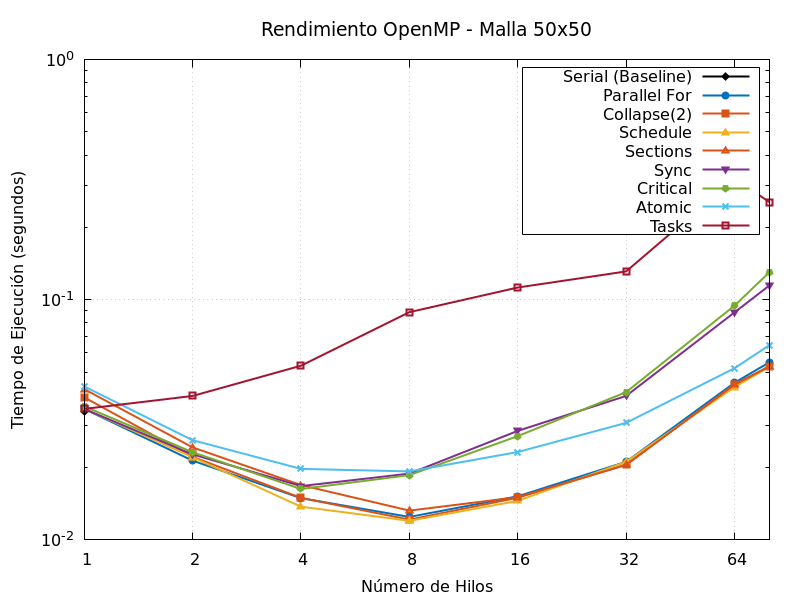
\includegraphics[width=0.49\linewidth]{../../imag/comparativa_malla_50.png}%
        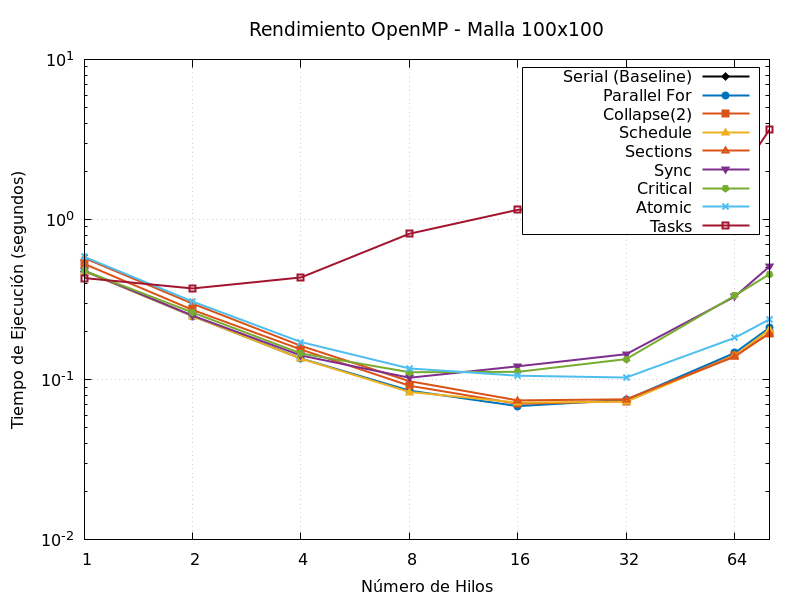
\includegraphics[width=0.49\linewidth]{../../imag/comparativa_malla_100.png}\\[2pt]
        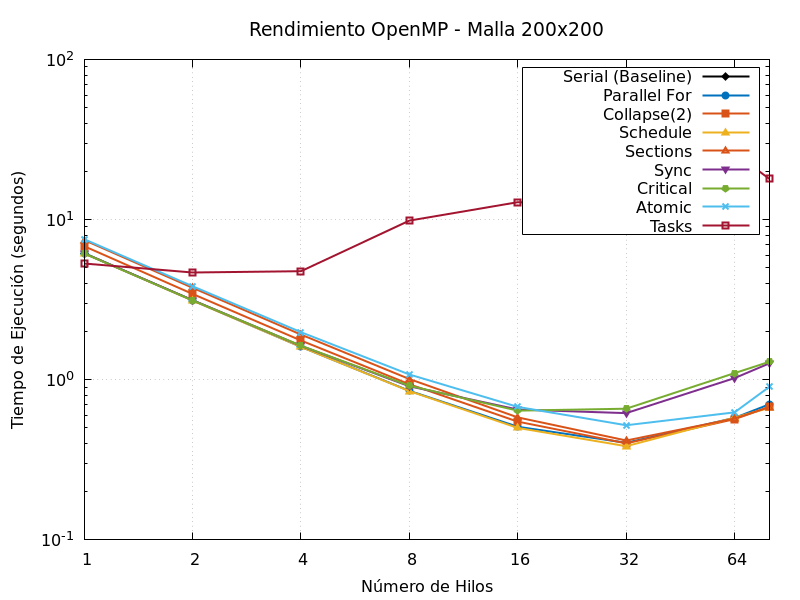
\includegraphics[width=0.70\linewidth]{../../imag/comparativa_malla_200.png}
      \end{figure}
    \column{0.34\textwidth}
      \begin{block}{Hallazgos Clave}
        \begin{itemize}
          \item El \emph{sweet spot} universal es \textbf{32 hilos}.
          \item Por encima de \textbf{64 hilos}: inflexión al alza.
          \item Causa: saturación del ancho de banda de la memoria compartida (\emph{Von Neumann Bottleneck}).
        \end{itemize}
      \end{block}
      \begin{alertblock}{Ley de Amdahl}
        $S(p)=\dfrac{1}{(1-\alpha)+\alpha/p}$\\[4pt]
        La fracción serial $\alpha$ limita la aceleración máxima teórica.
      \end{alertblock}
  \end{columns}
\end{frame}

% ============================================================
\section{Actividad 1 — \texttt{parallel for}}
% ============================================================

% <-- shrink=10 para encajar todo en la pag 7
\begin{frame}[fragile,shrink=10]{Act.\ 1 — \texttt{\#pragma omp parallel for}}
  \begin{columns}[t]
    \column{0.54\textwidth}
\begin{lstlisting}[language=C++,caption={Paralelización del bucle principal}]
#pragma omp parallel for reduction(max:delta)
for (int i = 1; i < M; ++i) {
  for (int j = 1; j < N; ++j) {
    double T_old = T[i][j];
    T[i][j] = (((T[i+1][j]+T[i-1][j])*k*k) + ((T[i][j+1]+T[i][j-1])*h*h)
              -(source[i][j]*h*h*k*k)) / (2.0*(h*h+k*k));
    double diff = abs(T[i][j]-T_old);
    if (diff > delta) delta = diff;
  }
}
iterations++;
\end{lstlisting}
      \begin{exampleblock}{¿Por qué \texttt{reduction(max:delta)}?}
        \begin{itemize}
            \item Evita \emph{data races} al sobreescribir \texttt{delta}.
            \item Garantiza un máximo local por hilo, combinado de forma segura al final.
        \end{itemize}
      \end{exampleblock}
    \column{0.44\textwidth}
      \begin{block}{Speedup en Malla $512^2$}
        \scriptsize
        \renewcommand{\arraystretch}{0.9}
        \begin{tabular}{@{}ccc@{}}
          \toprule
          \textbf{Hilos} & \textbf{Tiempo (s)} & \textbf{Speedup} \\
          \midrule
          1  & 177.86 & 1.00× \\
          4  & 44.77  & 3.97× \\
          16 & 11.81  & 15.06× \\
          32 & 6.63   & 26.82× \\
          \textbf{64} & \textbf{5.50} & \textbf{32.36×} \\
          \bottomrule
        \end{tabular}
      \end{block}
      \begin{alertblock}{Veredicto Arquitectónico}
        \textbf{Mejor costo-beneficio:} $32\times$ de \emph{speedup} con una sola línea de código.\\[4pt]
        Para 100\% de determinismo numérico, combinar con métodos de \emph{Jacobi} o \emph{Red-Black}.
      \end{alertblock}
  \end{columns}
\end{frame}

% ============================================================
\section{Actividad 2 — \texttt{collapse(2)}}
% ============================================================

\begin{frame}[fragile,shrink=8]{Act.\ 2 — \texttt{collapse(2)}: Fusión de Bucles}
  \begin{columns}[t]
    \column{0.50\textwidth}
\begin{lstlisting}[language=C++,caption={Espacio de iteración fusionado}]
#pragma omp parallel for collapse(2) reduction(max:delta)
for (int i = 1; i < M; ++i) {
  for (int j = 1; j < N; ++j) {
    // ... diferencias finitas ...
  }
}
\end{lstlisting}
      \begin{block}{¿Qué hace \texttt{collapse(2)}?}
        Fusiona bucles en un espacio lineal único de $(M{-}1)\times(N{-}1)$ iteraciones, aumentando la granularidad para el \emph{scheduler}.
      \end{block}
    \column{0.48\textwidth}
      \begin{block}{Comparativa vs \texttt{parallel for} ($512^2$, 64 hilos)}
        \scriptsize
        \renewcommand{\arraystretch}{0.9}
        \begin{tabular}{@{}lcc@{}}
          \toprule
          \textbf{Variante} & \textbf{Tiempo (s)} & \textbf{Speedup} \\
          \midrule
          \texttt{parallel for} & \textbf{5.50} & \textbf{32.36×} \\
          \texttt{collapse(2)}  & 5.83 & 30.52× \\
          \bottomrule
        \end{tabular}
      \end{block}
      \begin{alertblock}{¿Mejoró? \textbf{No.}}
        Introduce \emph{overhead} por el recálculo de índices. En mallas cuadradas donde $M \gg p$, el bucle externo ya es suficiente.
      \end{alertblock}
      \begin{exampleblock}{¿Cuándo sí usarlo?}
        Solo cuando el bucle externo tiene muy pocas iteraciones ($M \approx p$).
      \end{exampleblock}
  \end{columns}
\end{frame}

% ============================================================
\section{Actividad 3 — \texttt{sections}}
% ============================================================

\begin{frame}[fragile,shrink=8]{Act.\ 3 — \texttt{sections}: Inicialización en Paralelo}
  \begin{columns}[t]
    \column{0.50\textwidth}
\begin{lstlisting}[language=C++,caption={Bifurcación de inicialización}]
// Memoria reservada ANTES de la región paralela
std::vector<std::vector<double>> T(M+1, std::vector<double>(N+1, 0.0));
std::vector<std::vector<double>> source(M+1, std::vector<double>(N+1, 0.0));

#pragma omp parallel sections
{
  #pragma omp section
  initialize_boundaries(M, N, T, h, k);

  #pragma omp section
  poisson_source(M, N, source);
}
\end{lstlisting}
    \column{0.48\textwidth}
      \begin{block}{Speedup Malla $512^2$ (Total)}
        \scriptsize
        \renewcommand{\arraystretch}{0.9}
        \begin{tabular}{@{}ccc@{}}
          \toprule
          \textbf{Hilos} & \textbf{Tiempo (s)} & \textbf{Speedup} \\
          \midrule
          1  & 177.86 & 1.00× \\
          16 & 14.06  & 12.65× \\
          64 & 6.03   & 29.50× \\
          \bottomrule
        \end{tabular}
      \end{block}
      \begin{alertblock}{¿Tuviste que reordenar? \textbf{Sí}}
        Para evitar \emph{Seg-Faults}, la memoria debe asignarse estáticamente en el hilo maestro.
      \end{alertblock}
      \begin{alertblock}{¿Vale la pena? \textbf{No}}
        \begin{itemize}
            \item Inicialización $\mathcal{O}(N^2)$ es trivial.
            \item El \emph{overhead} de fork-join excede el beneficio.
            \item Ideal solo para I/O asimétrico.
        \end{itemize}
      \end{alertblock}
  \end{columns}
\end{frame}

% ============================================================
\section{Actividad 4 — \texttt{schedule}}
% ============================================================

\begin{frame}[fragile,shrink=10]{Act.\ 4 — Control Explícito y \texttt{schedule}}
  \begin{columns}[t]
    \column{0.50\textwidth}
\begin{lstlisting}[language=C++,caption={Región paralela separada del bucle}]
#pragma omp parallel // Fork explícito
{
  #pragma omp for schedule(static) reduction(max:delta)
  for (int i = 1; i < M; ++i) {
    for (int j = 1; j < N; ++j) {
      // Discretización de Poisson
    }
  }
} // Join implícito
\end{lstlisting}
      \begin{exampleblock}{\texttt{static} vs \texttt{dynamic}}
        \begin{itemize}
            \item \textbf{\texttt{static}:} Reparto en compilación. Ideal para FLOPs uniformes (como Poisson).
            \item \textbf{\texttt{dynamic}:} Reparto en ejecución. Ideal para cargas desbalanceadas.
        \end{itemize}
      \end{exampleblock}
    \column{0.48\textwidth}
      \begin{block}{Speedup Malla $512^2$ — \texttt{schedule(static)}}
        \scriptsize
        \renewcommand{\arraystretch}{0.9}
        \begin{tabular}{@{}ccc@{}}
          \toprule
          \textbf{Hilos} & \textbf{Tiempo (s)} & \textbf{Speedup} \\
          \midrule
          1  & 177.86 & 1.00×  \\
          16 & 11.78  & 15.10× \\
          32 & 6.72   & 26.46× \\
          \textbf{64} & \textbf{5.55} & \textbf{32.06×} \\
          \bottomrule
        \end{tabular}
      \end{block}
      \begin{alertblock}{Por qué NO se usó \texttt{dynamic}}
        Cada celda ejecuta la misma carga. Forzar asignación dinámica inunda el bus con \emph{overhead} de control.
      \end{alertblock}
      \begin{exampleblock}{Ventaja \texttt{parallel} + \texttt{for}}
        No recrear el equipo de hilos en cada iteración del \texttt{while} reduce latencia acumulada.
      \end{exampleblock}
  \end{columns}
\end{frame}

% ============================================================
\section{Actividad 5 — Sincronización Explícita}
% ============================================================

\begin{frame}[fragile,shrink=12]{Act.\ 5 — \texttt{nowait, barrier, single, critical}}
  \begin{columns}[t]
    \column{0.50\textwidth}
\begin{lstlisting}[language=C++,caption={Sincronización manual}]
double local_delta = 0.0;

#pragma omp for nowait
for (int i = 1; i < M; ++i)
  for (int j = 1; j < N; ++j) {
    /* calc diff */
    if (diff>local_delta) local_delta=diff;
  }

#pragma omp critical
{ if (local_delta > delta) delta = local_delta; }

#pragma omp barrier

#pragma omp single
{ iterations++; }
\end{lstlisting}
    \column{0.48\textwidth}
      \begin{block}{Resultados — Malla $512^2$}
        \scriptsize
        \renewcommand{\arraystretch}{0.9}
        \begin{tabular}{@{}ccc@{}}
          \toprule
          \textbf{Hilos} & \textbf{Tiempo (s)} & \textbf{Speedup} \\
          \midrule
          1  & 177.86 & 1.00×  \\
          16 & 12.24  & 14.52× \\
          64 & 7.13   & 24.94× \\
          \bottomrule
        \end{tabular}
      \end{block}
      \begin{alertblock}{\texttt{nowait}: ¿hubo cambio?}
        El beneficio fue anulado por el embotellamiento del \texttt{critical} y la \texttt{barrier} posterior. Peor que \texttt{reduction}.
      \end{alertblock}
      \begin{block}{Roles Clave}
        \begin{itemize}
          \item \textbf{\texttt{single}:} Evita que \texttt{iterations} sume $p$ veces por barrido.
          \item \textbf{\texttt{critical}:} Solo para estructuras complejas no soportadas por hardware.
        \end{itemize}
      \end{block}
  \end{columns}
\end{frame}

% ============================================================
\section{Actividad 6 — \texttt{critical} vs \texttt{atomic}}
% ============================================================

\begin{frame}[fragile,shrink=10]{Act.\ 6 — \texttt{critical} vs \texttt{atomic}: Software vs Hardware}
  \begin{columns}[t]
    \column{0.48\textwidth}
\begin{lstlisting}[language=C++,caption={Sincronización escalares}]
// Estrategia 1: Software
#pragma omp critical(update_delta)
{
  if (local_delta > delta) delta = local_delta;
}

// Estrategia 2: Hardware
#pragma omp atomic
iterations++;
\end{lstlisting}
      \begin{block}{Mecanismo Interno}
        \begin{itemize}
            \item \textbf{\texttt{critical}:} Mutexes del S.O. Genera \emph{context switch} (costoso).
            \item \textbf{\texttt{atomic}:} Instrucciones nativas en chip (Ej. \texttt{LOCK INC}). Ejecuta en \textbf{$\sim$3-5 ciclos}.
        \end{itemize}
      \end{block}
    \column{0.50\textwidth}
      \begin{block}{Alta Concurrencia (64 hilos)}
        \scriptsize
        \renewcommand{\arraystretch}{0.9}
        \begin{tabular}{@{}cccc@{}}
          \toprule
          \textbf{Malla} & \textbf{\texttt{critical} (s)} & \textbf{\texttt{atomic} (s)} & \textbf{Mejora} \\
          \midrule
          $64^2$   & 0.169 & \textbf{0.092} & +45\% \\
          $128^2$  & 0.479 & \textbf{0.278} & +41\% \\
          $256^2$  & 1.946 & \textbf{1.208} & +38\% \\
          $512^2$  & 7.847 & \textbf{6.605} & +15\% \\
          \bottomrule
        \end{tabular}
      \end{block}
      \begin{exampleblock}{Regla General}
        \textbf{\texttt{atomic}} siempre para contadores/sumas simples. \textbf{\texttt{critical}} solo para bloques multilínea o memoria dispersa.
      \end{exampleblock}
      \begin{alertblock}{Nota Arquitectónica}
        Usar \texttt{atomic} dentro de \texttt{single} es redundante. Brilla cuando hay concurrencia real sin control único.
      \end{alertblock}
  \end{columns}
\end{frame}

% ============================================================
\section{Actividad 7 — \texttt{task}}
% ============================================================

\begin{frame}[fragile,shrink=12]{Act.\ 7 — Paralelismo de Tareas (\texttt{task})}
  \begin{columns}[t]
    \column{0.50\textwidth}
\begin{lstlisting}[language=C++,caption={División por bloques}]
const int BS = 16; // Block Size
#pragma omp parallel shared(T,source,delta)
{
  #pragma omp single
  {
    for (int bi=1; bi<M; bi+=BS)
      for (int bj=1; bj<N; bj+=BS)
        #pragma omp task firstprivate(bi,bj) shared(T,delta)
        {
          double loc_d = 0.0;
          for (int i=bi; i<min(bi+BS,M); i++)
            for (int j=bj; j<min(bj+BS,N); j++)
            { /* calc diff */ }
          
          #pragma omp critical
          if (loc_d > delta) delta = loc_d;
        }
  } // taskwait implícito
  iterations++;
}
\end{lstlisting}
    \column{0.48\textwidth}
      \begin{alertblock}{Colapso de Rendimiento ($512^2$)}
        \scriptsize
        \renewcommand{\arraystretch}{0.9}
        \begin{tabular}{@{}cccc@{}}
          \toprule
          \textbf{Hilos} & \textbf{Tiempo (s)} & \textbf{Speedup} \\
          \midrule
          4  & 124.3  & 1.43× \\
          32 & 319.4  & 0.55× \\
          64 & \textbf{589.7} & \textbf{0.30×} \\
          \midrule
          \multicolumn{3}{@{}c@{}}{\textbf{\texttt{parallel for} base:} 5.50 s (32.36×)} \\
          \bottomrule
        \end{tabular}
      \end{alertblock}
      \begin{alertblock}{¿Por qué es $\approx 100\times$ más lento?}
        Bloques $16\times16$ generan $\mathbf{1\,024}$ tareas \textbf{por iteración temporal}. El \emph{scheduler} colapsa encolando y despachando, no calculando.
      \end{alertblock}
      \begin{exampleblock}{¿Cuándo sí usar \texttt{task}?}
        Estructuras irregulares: grafos, árboles, recursividad. Matrices densas $\rightarrow$ \texttt{parallel for}.
      \end{exampleblock}
  \end{columns}
\end{frame}

% ============================================================
\section{Comparación Final}
% ============================================================

\begin{frame}{Tabla Comparativa — Malla $512\times512$, 64 Hilos}
  \begin{center}
  \scriptsize
  \renewcommand{\arraystretch}{1.1}
  \begin{tabularx}{\textwidth}{@{}l l c c X@{}}
    \toprule
    \textbf{Versión} & \textbf{Directiva} & \textbf{Tiempo} & \textbf{Speedup} & \textbf{Diagnóstico HPC} \\
    \midrule
    Secuencial        & N/A                  & 177.86 s  & 1.00×   & Baseline de normalización. \\
    \rowcolor{UDlight}
    \textbf{Parallel For} & \texttt{parallel for} & \textbf{5.48 s} & \textbf{32.5×} & \textbf{Superior.} Balance óptimo. \\
    Schedule          & \texttt{schedule}    & 5.52 s    & 32.1×   & Equivalente al básico. Estático ideal. \\
    Collapse          & \texttt{collapse(2)} & 5.78 s    & 30.7×   & Leve penalización por índices lineales. \\
    Sections          & \texttt{sections}    & 6.00 s    & 29.6×   & Fork-join no justificado para $O(N^2)$. \\
    Atomic            & \texttt{atomic}      & 6.61 s    & 26.9×   & Sincronización eficiente en hardware. \\
    Critical          & \texttt{critical}    & 7.13 s    & 24.9×   & Penalización por \emph{lock contention}. \\
    \rowcolor{UDsecond!15}
    \textbf{Tareas}   & \texttt{task}        & 117.5 s   & 1.51×   & \textbf{Colapso.} Planificador asfixiado. \\
    \bottomrule
  \end{tabularx}
  \end{center}
  \vspace{0.2cm}
  \begin{columns}[t]
    \column{0.48\textwidth}
      \begin{exampleblock}{Regla de Oro}
        Para EDPs en dominios regulares:\\
        \textbf{parallel for + reduction} $\gg$ todo lo demás.
      \end{exampleblock}
    \column{0.48\textwidth}
      \begin{alertblock}{Trampa Frecuente}
        Más hilos $\neq$ más \emph{speedup}. El \emph{overhead} domina si la carga por hilo es minúscula.
      \end{alertblock}
  \end{columns}
\end{frame}

% ============================================================
\section{Validación Numérica}
% ============================================================

\begin{frame}{Validación Numérica de la Solución}
  \begin{columns}[c]
    \column{0.52\textwidth}
      \begin{figure}
        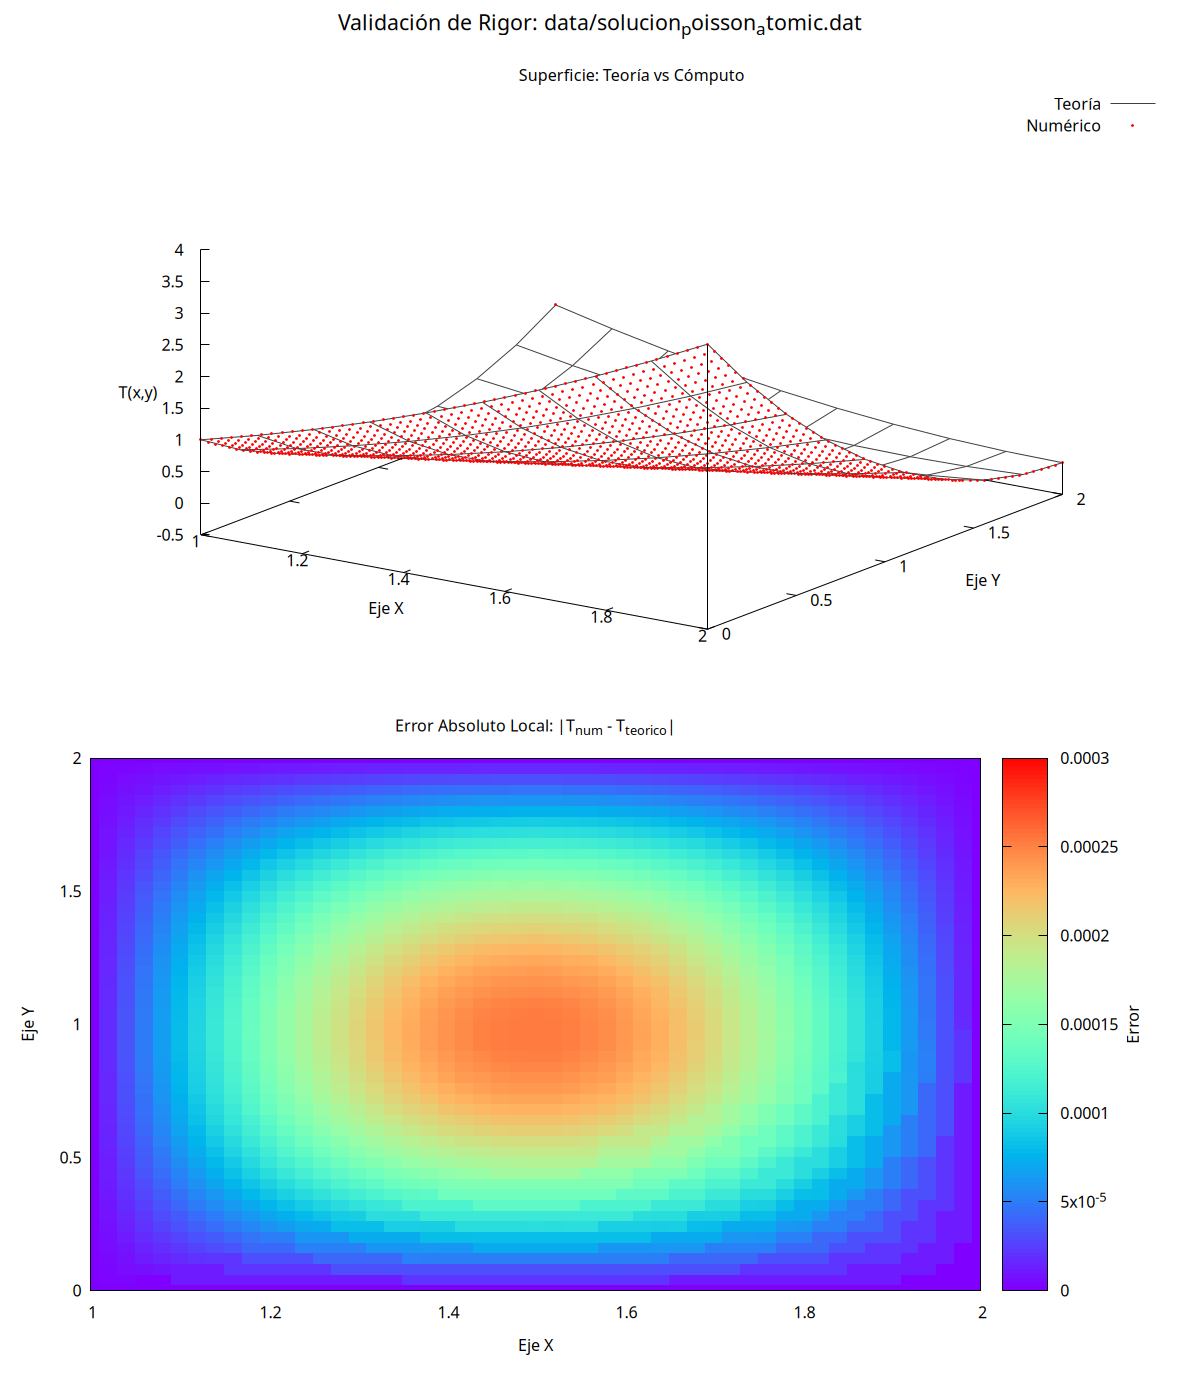
\includegraphics[width=0.75\linewidth]{../../imag/solucion_poisson_atomic.png}
        \caption{Solución $50\times50$ (\texttt{atomic}).}
      \end{figure}
    \column{0.46\textwidth}
      \begin{figure}
        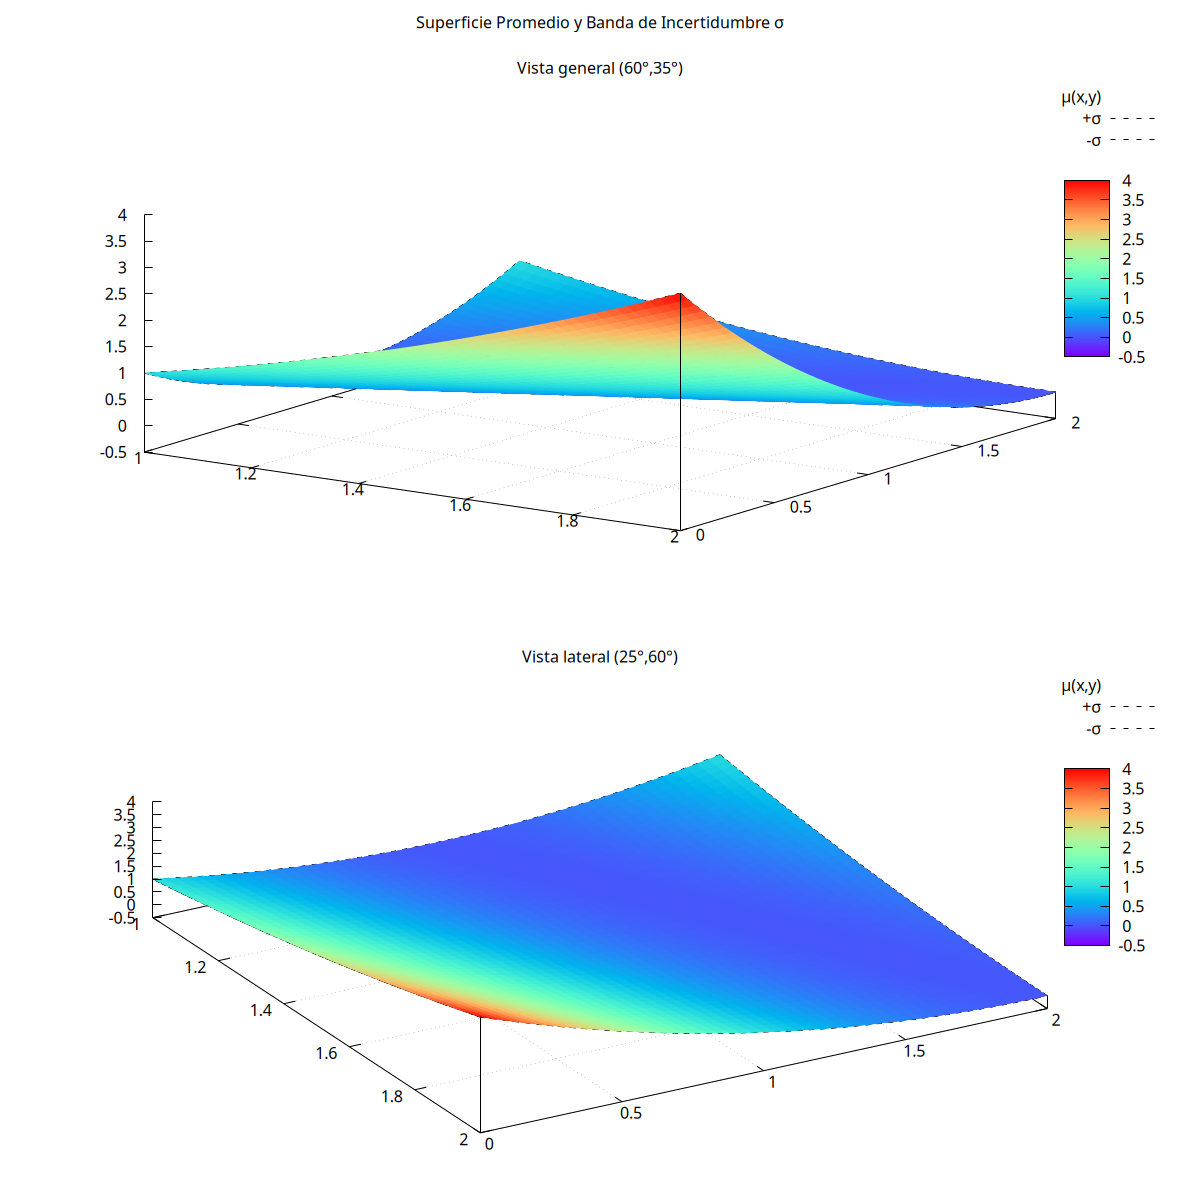
\includegraphics[width=0.90\linewidth]{../../imag/validacion_stats.png}
        \caption{Desviación estándar (7 métodos).}
      \end{figure}
  \end{columns}
  \vspace{0.2cm}
  \begin{columns}[t]
    \column{0.48\textwidth}
      \begin{block}{Forma Esperada}
        Reproduce la \textbf{parábola} teórica dictada por Dirichlet y $f=4$. Error global $< 10^{-6}$.
      \end{block}
    \column{0.48\textwidth}
      \begin{exampleblock}{Invarianza Numérica}
        Todas las implementaciones convergen a la \emph{misma solución}. Las variaciones son puramente \textbf{computacionales}.
      \end{exampleblock}
  \end{columns}
\end{frame}

% ============================================================
\section{Conclusiones}
% ============================================================

\begin{frame}[shrink=10]{Conclusiones Generales}
  \begin{columns}[t]
    \column{0.49\textwidth}
      \begin{block}{1. Paradigma Dominante}
        \begin{itemize}
            \item \texttt{parallel for + reduction} es superior.
            \item La uniformidad geométrica permite distribución estática ideal.
            \item \textbf{Speedup máx:} $32.5\times$ (64 hilos, malla $512^2$).
        \end{itemize}
      \end{block}

      \begin{block}{2. Costo de Sincronización}
        \begin{itemize}
          \item Hardware (\texttt{atomic}): $\sim$6.6 s
          \item Software (\texttt{critical}): $\sim$7.1 s
          \item Preferir siempre \texttt{atomic}.
        \end{itemize}
      \end{block}
    \column{0.49\textwidth}
      \begin{alertblock}{3. Falla del Modelo de Tareas}
        \begin{itemize}
            \item El \emph{runtime} colapsa encolando 1,024 tareas/iteración.
            \item Rendimiento $117\times$ peor que \texttt{parallel for}.
            \item Usar solo para grafos o recursividad.
        \end{itemize}
      \end{alertblock}

      \begin{exampleblock}{4. Validez Numérica}
        \begin{itemize}
            \item La paralelización \textbf{no afecta la física}.
            \item 100\% de consistencia en el esquema de diferencias finitas iterativo.
        \end{itemize}
      \end{exampleblock}
  \end{columns}

  \vspace{0.3cm}
  \begin{center}
    \begin{tikzpicture}
      \node[fill=UDprimary,text=white,rounded corners=4pt,
            inner xsep=12pt,inner ysep=6pt,font=\bfseries\small] {
        Veredicto final: \texttt{parallel for} con \texttt{reduction} es la solución óptima para EDPs.
      };
    \end{tikzpicture}
  \end{center}
\end{frame}

% ─── DIAPOSITIVA DE CIERRE ────────────────────────────────────
{
\setbeamertemplate{headline}{}
\setbeamertemplate{footline}{}
\begin{frame}[plain]
  \begin{tikzpicture}[remember picture,overlay]
    \fill[UDprimary] (current page.south west) rectangle (current page.north east);
    \fill[UDdark,opacity=0.4]
      (current page.south west) rectangle (current page.north east);
    \fill[UDsecond,opacity=0.85]
      ([xshift=-0.08\paperwidth]current page.north east) rectangle
      (current page.south east);
    \draw[UDlight,line width=1.5pt]
      ([yshift=-0.45\paperheight]current page.north west) --
      ([yshift=-0.45\paperheight,xshift=-0.08\paperwidth]current page.north east);
  \end{tikzpicture}

  \begin{center}
    \vspace{0.8cm}
    {\color{white}\Huge\bfseries ¡Gracias!}\\[10pt]
    \color{white}\rule{0.5\textwidth}{0.4pt}\\[10pt]
    {\color{UDlight}\large Camilo Huertas \quad · \quad Sebastián Rodriguez}\\[6pt]
    {\color{UDlight}\small Programa Académico de Física}\\
    {\color{UDlight}\small Universidad Distrital Francisco José de Caldas}\\[6pt]
    {\color{UDlight}\footnotesize Docente: Carlos Andrés Gómez Vasco \quad|\quad Sistemas Distribuidos}
  \end{center}
\end{frame}
}

\end{document}
